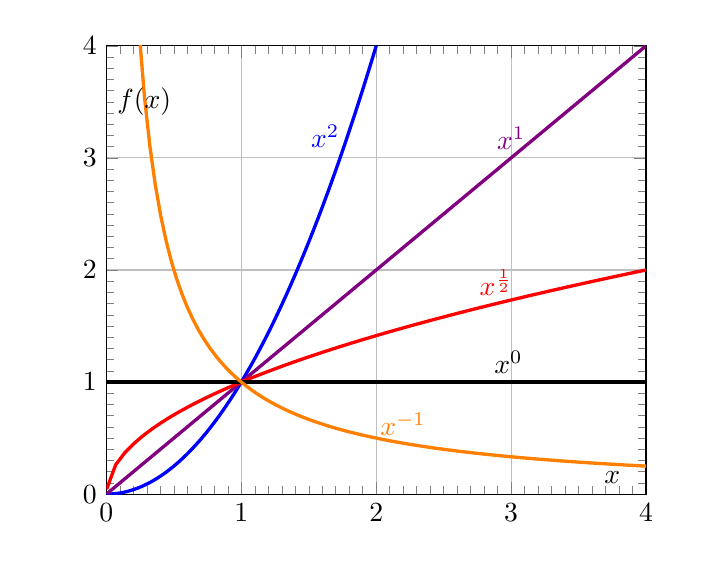
\begin{tikzpicture}
    % invisible boundbox
    \draw[draw=none](-1,-0.6) rectangle (+7.2,+5.9);
\begin{axis}[
    %title={Potenzfunktionen $x^n$, lineare Skalen},% außerhalb der boundbox
    xmode=linear, ymode=linear,% normal|linear|log
    xmin = 0, xmax = 4,
    ymin = 0, ymax = 4,
    domain = 0.002:4,
    samples=61,
    xtick distance=1,
    ytick distance=1,
    minor x tick num=9,
    minor y tick num=9,
    grid=major,
]
    \addplot+[mark=none,very thick, blue,domain=0:2] {x^2}  node[pos=0.82,anchor=east,xshift=+1pt] {$x^2$};
    \addplot+[mark=none,very thick, violet] {x}             node[pos=0.75,anchor=south,yshift=-1pt] {$x^1$};
    \addplot+[mark=none, very thick, red] {x^0.5}           node[pos=0.75,anchor=south,yshift=-1pt] {$x^{\frac{1}{2}}$};
    \addplot+[mark=none, very thick, black] {1}             node[pos=0.75,anchor=south,yshift=-1pt,xshift=-1pt] {$x^{0}$};
    \addplot+[mark=none, very thick, orange, samples=101,
        restrict y to domain=0:5] {x^-1}  node[pos=0.75,anchor=south,yshift=-1pt] {$x^{-1}$};
    % axis labels inside plot
    \addplot[mark=none, very thick, black] coordinates {(3.75,0.00)} node[anchor=south] {$x$}; % xlabel
    \addplot[mark=none, very thick, black] coordinates {(0.00,3.50)} node[anchor=west] {$f(x)$}; % ylabel
    %\addplot[mark=none, very thick, black, ->] coordinates {(0.75,0.10)(1.25,0.10)} node[pos=0.5,anchor=south] {$x$}; % xlabel
    %\addplot[mark=none, very thick, black, ->] coordinates {(0.05,2.50)(0.05,3.50)} node[pos=0.5,anchor=west] {$f(x)$}; % ylabel
\end{axis}
\end{tikzpicture}